\documentclass[11pt]{article}
\usepackage[margin=1in]{geometry}
\usepackage{amsmath,amssymb,amsthm}
\usepackage{graphicx}
\usepackage{booktabs}
\usepackage{hyperref}
\usepackage{algorithm}
\usepackage{algorithmic}
\usepackage{subcaption}
\usepackage{xcolor}

\title{GNNs vs.\ Proven Approximation Algorithms:\\A Rigorous Empirical Audit on NP-Hard Problems}
\author{Alan Zhang}
\date{June 2026}

\begin{document}
\maketitle

\begin{abstract}
Graph Neural Networks (GNNs) have been proposed as learned solvers for NP-hard combinatorial optimization problems, yet their performance relative to classical algorithms with \emph{proven approximation guarantees} remains poorly characterized.
We conduct a rigorous empirical audit comparing GIN-based GNN solvers against classical algorithms on three canonical NP-hard problems: Maximum Cut, Travelling Salesman Problem, and Graph Coloring.
An ablation-driven audit of our own initial Max-Cut pipeline produced the decisive finding: with constant node features, the unsupervised cut loss has an exact critical point at the uniform output whose value is precisely the random-cut baseline, so a naively-trained GNN is indistinguishable from a coin flip that receives the same local-search refinement (mean ratio 0.990 between the two), and the network's raw output is \emph{worse} than a coin flip (0.21 vs.\ \textasciitilde0.50 of edges cut) --- echoing the critique Angelini \& Ricci-Tersenghi and Boettcher levelled at Schuetz et al.'s PI-GNN.
Rebuilt with symmetry-breaking Laplacian positional-encoding features, an $O(1)$ logit initialisation, a best-of-50 Bernoulli decoding matched to the Goemans-Williamson rounding budget, an edge-count-normalised loss, and per-graph normalisation, the same 5-layer GIN becomes a credible heuristic on 600 held-out instances: it beats a budget-matched coin-flip control (best-of-50 coin flips + the same local search; mean ratio 1.038, 95\% CI [1.035, 1.041]) and the spectral method (1.008 [1.006, 1.010]), but still loses to Goemans-Williamson (0.987 [0.985, 0.988]) --- and GW refined with the same local search finds the exact optimum on 299 of the 300 instances verified so far ($n \leq 20$).
We report win/tie/loss three-ways, approximation ratios with paired-bootstrap confidence intervals, Wilcoxon signed-rank tests, and in-distribution vs.\ out-of-distribution splits across three training seeds.
For TSP, NN+2-opt local search matches or outperforms the GNN+2-opt on all 90 Euclidean instances; for Graph Coloring the GNN genuinely loses (0 wins / 3 ties / 597 losses, 15.4 vs.\ 5.4 mean colours against DSatur).
The GNN's primary advantage is inference speed, not solution quality.
These results demonstrate that for practitioners, classical algorithms with mathematical guarantees remain the reliable baseline, and that learned pipelines must be ablated against the classical post-processing they contain before any claim about the learned component is made.
\end{abstract}

\section{Introduction}

Combinatorial optimization over graphs---finding optimal cuts, shortest tours, minimal colorings---is a cornerstone of both computer science theory and applied operations research.
Many of these problems are NP-hard \cite{garey1979computers}, meaning no polynomial-time algorithm can solve all instances exactly (unless P~=~NP).
However, decades of work in approximation algorithms have produced remarkable results: polynomial-time algorithms with \emph{provable} worst-case guarantees on solution quality \cite{vazirani2001approximation}.

Recent years have seen growing interest in using Graph Neural Networks (GNNs) to learn solvers for these problems \cite{khalil2017learning, bengio2021machine, cappart2023combinatorial}.
The appeal is clear: GNNs can leverage structural patterns in graph data, amortize computation across instances, and potentially discover heuristics that exploit distributional regularity.

However, a troubling gap exists in the literature: GNN solvers are typically compared against simple baselines (random, greedy) rather than against the best classical algorithms with known guarantees.
This creates an inflated impression of GNN effectiveness.
A GNN that beats a random partition on Max-Cut is unremarkable; one that beats the Goemans-Williamson SDP relaxation \cite{goemans1995improved} would be extraordinary.

\textbf{Contributions.} We provide a rigorous empirical audit comparing GNN solvers against the strongest classical algorithms on three problems, with ablations that isolate where performance actually comes from:

\begin{enumerate}
    \item \textbf{Maximum Cut}: GNN (GIN + shared local search) vs.\ Goemans-Williamson SDP ($\alpha \geq 0.878$), spectral relaxation, greedy, and a coin-flip control with the identical refinement, across 600 instances from 5 graph families, three training seeds, with paired-bootstrap CIs and exact optima for $n \leq 20$.
    \item \textbf{Travelling Salesman Problem}: GNN vs.\ Christofides ($\alpha \leq 1.5$) and 2-opt local search, on 90 Euclidean instances.
    \item \textbf{Graph Coloring}: GNN vs.\ DSatur \cite{brelaz1979new} and Welsh-Powell, across 600 instances from 5 graph families.
    \item \textbf{Failure Prediction}: We train classifiers on spectral graph properties to predict when the GNN pipeline wins. With 11.3\% positive examples the task remains at chance (LR balanced accuracy 0.54 $\pm$ 0.18, F1 0.21) --- too little signal to support a reliable predictor.
    \item \textbf{A negative-control ablation} showing that a naively-trained GNN's apparent performance is almost entirely the classical post-processing it contains, and an analysis of \emph{why} (a provable critical point of the loss at the uniform output), with the architectural fixes that turn the network into a credible heuristic.
\end{enumerate}

\section{Background}

\subsection{Approximation Algorithms and Guarantees}

An $\alpha$-approximation algorithm for a maximization problem produces a solution of value $\geq \alpha \cdot \text{OPT}$ in polynomial time.
For minimization, $\leq \alpha \cdot \text{OPT}$.

\textbf{Max-Cut.} Given a graph $G = (V, E)$, find a partition $(S, V \setminus S)$ maximizing the number of edges crossing the cut.
The Goemans-Williamson algorithm \cite{goemans1995improved} solves an SDP relaxation and rounds via random hyperplanes, achieving $\alpha \geq 0.878$.
Under the Unique Games Conjecture, this is optimal.

\textbf{TSP.} Given $n$ cities with pairwise distances satisfying the triangle inequality, find the shortest Hamiltonian tour.
The Christofides-Serdyukov algorithm \cite{christofides1976worst} computes an MST, adds a minimum-weight perfect matching on odd-degree vertices, and shortcuts the resulting Eulerian tour, achieving $\alpha \leq 1.5$.
This stood as the best known approximation for nearly 50 years.

\textbf{Graph Coloring.} Given a graph, assign colors to vertices such that no adjacent vertices share a color, minimizing the number of colors.
This problem is notoriously hard to approximate: for any $\epsilon > 0$, it is NP-hard to color a 3-colorable graph with $n^{1-\epsilon}$ colors.
DSatur \cite{brelaz1979new} is a widely-used heuristic that is optimal for bipartite graphs.

\subsection{Graph Neural Networks for Combinatorial Optimization}

GNNs learn to map graph-structured inputs to node or edge-level predictions through message-passing layers \cite{xu2019powerful}.
For combinatorial optimization, the typical approach is unsupervised: the GNN outputs soft assignments (e.g., partition probabilities for Max-Cut), trained with a loss that directly encodes the objective \cite{khalil2017learning, karalias2020erdos, schuetz2022combinatorial}.
This line of work is contested. Angelini and Ricci-Tersenghi \cite{angelini2023modern} showed that a near-linear-time greedy algorithm beats Schuetz et al.'s physics-inspired GNN (PI-GNN) \cite{schuetz2022combinatorial} on maximum \emph{independent set}; Boettcher \cite{boettcher2023inability} raised the same concern for the PI-GNN approach against greedy and gradient-descent baselines. Their problem differs from ours (MIS vs.\ Max-Cut, and their PI-GNN is a per-instance relaxation, not a trained generalising model), but the shared lesson --- that apparent GNN performance can be an artefact of weak baselines or of classical post-processing attached to the learned pipeline --- is exactly what our ablation reproduces from the inside.
Our audit reaches the same conclusion from the inside, by ablating our own pipeline down to a coin-flip control.

We use the Graph Isomorphism Network (GIN) \cite{xu2019powerful} throughout, as it is as expressive as the 1-WL test (the most expressive \emph{standard} message-passing GNN; higher-order GNNs are strictly more expressive).
Karalias and Loukas \cite{karalias2020erdos} derive probabilistic penalty losses whose decoding samples from the learned per-node distribution --- the best-of-many-rounding scheme we adopt for decoding.

\section{Experimental Setup}

\subsection{Graph Families}

We test generalization by training on one family and evaluating on five:
\begin{itemize}
    \item \textbf{Erd\H{o}s-R\'enyi} $G(n, p)$: random edges with $p = 0.15$
    \item \textbf{Planted Partition}: stochastic block model with 2 communities
    \item \textbf{Random Regular}: $d$-regular graphs ($d = 3$)
    \item \textbf{Barab\'asi-Albert}: preferential attachment ($m = 3$)
    \item \textbf{Watts-Strogatz}: small-world ($k = 4$, $p = 0.3$)
\end{itemize}

Graph sizes: $n \in \{20, 50, 100, 200\}$, with 30 instances per (family, size) pair, totaling 600 instances per problem.

\subsection{GNN Architecture, and the Three Fixes}

All GNN solvers use a 5-layer GIN with 128-dimensional hidden states.
For Max-Cut, the output is a per-node sigmoid probability; for Coloring, a softmax over 20 possible colors; for TSP, node embeddings scored by dot product.

An external ablation audit of the \emph{original} Max-Cut configuration (constant node features, unnormalised loss, BatchNorm, single-threshold decoding) found it effectively broken: the network's raw output was worse than a coin flip and nearly all measured performance came from the attached local search. The Max-Cut model was rebuilt with three fixes, in order of measured impact:

\begin{itemize}
    \item \textbf{Symmetry-breaking features.} With constant features, the loss has an exact critical point at the uniform output $p \equiv 0.5$ --- its (unnormalised) value is exactly $|E|/2$, the random-cut baseline, and a deterministic message-passing net cannot distinguish nodes there. The Max-Cut GIN now receives Laplacian positional encodings (the node's normalised degree plus its coordinates in the top-4 eigenvectors of $L$, sign-canonicalised), which survive neighbourhood aggregation. We tried two alternatives and discarded them (reproduced by \texttt{run\_gnn\_symmetry\_diagnostics.py}): a constant-feature GIN's output is near-constant across nodes and its thresholded partition is degenerate (empty or all-one-side) on about a third of sampled instances, and plain LayerNorm shrinks the across-node signal monotonically over five layers whereas per-graph GraphNorm keeps it roughly constant. Note that the top eigenvector is essentially the spectral baseline's partition; the GNN is therefore \emph{given} the spectral answer and asked to refine it, not to discover it (see the caveats).
    \item \textbf{Matched decoding budget.} The original decoder thresholded one deterministic forward pass at $p>0.5$ (with a degenerate-output guard). The rebuilt decoder samples the partition as Bernoulli($p$) coin flips 50 times and keeps the best cut --- the same best-of-many rounding budget the Goemans-Williamson solver receives, in the spirit of the probabilistic decoding of \cite{karalias2020erdos}.
    \item \textbf{Loss normalisation and per-graph statistics.} The loss is divided by the number of (undirected) edges so it reads directly as the fraction of edges cut and is comparable across configurations; BatchNorm is replaced by per-graph GraphNorm so no statistics fitted on the training distribution are ever applied to a test graph.
\end{itemize}

The rebuilt model is trained with a 10\% held-out validation slice, checkpoint selection on validation loss, and cosine LR annealing, on three seeds (42, 43, 44); the canonical committed run is seed 42 and the seed spread is reported.
The TSP and Coloring models keep their original architectures (their committed artifacts are from the original runs).

\subsection{Evaluation Protocol}

Each algorithm is evaluated on: (1) solution quality as the mean approximation ratio and mean cut per edge, (2) wall-clock time, and (3) win/tie/loss three-ways against every other method.
Every method --- including a coin flip --- receives the same optional 1-opt local-search refinement, so the comparison isolates the learned component; the pairwise head-to-heads are additionally reported with paired-bootstrap 95\% CIs and Wilcoxon signed-rank tests.
For $n \leq 20$ the exact optimum is computed by brute force ($2^n$ enumeration), turning relative comparisons into rigorous ones.
All experiments run on CPU (Apple M3) for timing comparison; GNN timings exclude training cost (amortisation is discussed in the caveats).

\subsection*{Erratum}

A post-publication audit found that the original evaluation seeds (\texttt{42 + 1000\,i}) placed two of the 600 Max-Cut instances (Erd\H{o}s--R\'enyi, $n{=}100$, seeds 42 and 1042) inside the training seed range 42--2041: two evaluation graphs had been seen during training. The experiment runner now offsets evaluation seeds beyond the training range (\texttt{42 + 2000 + 1000\,i}), and the comparison was regenerated end to end under the fixed runner. The same audit prompted three reporting fixes in the repository: exact ties are now reported alongside wins and losses; a \texttt{gw\_fallback} column records whenever Goemans-Williamson substituted the spectral relaxation; and the failure-prediction scaler is now fitted inside each cross-validation fold.

A second, ablation-focused audit then found the decisive issue addressed in this revision: the original GNN pipeline's apparent performance was almost entirely its attached local search (a coin flip with the identical refinement scored within 1\% of the pipeline), with the network's raw output worse than a coin flip --- a provable consequence of the constant-feature critical point described above. The Max-Cut model was rebuilt with the three fixes, retrained on three seeds, and every comparison re-run end to end under the committed runners; the committed artifacts are the regenerated outputs.

\section{Results}

\subsection{Maximum Cut}
\label{sec:maxcut}

\begin{table}[h]
\centering
\caption{Max-Cut results across 600 committed-run instances (5 families $\times$ 4 sizes $\times$ 30). Every learned or constructed partition may be refined by the same 1-opt local search. Win/tie/loss = strict comparison against every other method. GNN row: the rebuilt model, canonical (seed-42) run.}
\label{tab:maxcut}
\begin{tabular}{lcccc}
\toprule
\textbf{Algorithm} & \textbf{Guarantee} & \textbf{Avg Cut/Best} & \textbf{Win/Tie/Loss} & \textbf{Avg Time (s)} \\
\midrule
Random partition & $\geq 0.5$ & 0.671 & 0\%/0\%/100\% & $< 0.001$ \\
Greedy local search & $\geq 0.5$ & 0.945 & 0\%/4.8\%/95.2\% & 0.002 \\
Spectral (+ its LS) & --- & 0.979 & 2.0\%/19.2\%/78.8\% & 0.003 \\
Goemans-Williamson & $\geq 0.878$ & \textbf{0.999} & 0\%/51.7\%/48.3\%$^{a}$ & 3.6 \\
\textbf{GNN (rebuilt) + shared LS} & --- & 0.986 & 2.0\%/25.5\%/72.5\% & 0.037 \\
\bottomrule
\end{tabular}
\caption*{\footnotesize $^{a}$GW loses only to GW+LS, which refines GW's own output (Table~\ref{tab:ablation}).
Avg times are wall-clock means over the committed run on one machine, dominated by the $n{=}200$ SDP solves;
runtimes are environment- and threading-dependent and are reported only to show ordering.}
\end{table}

\begin{table}[h]
\centering
\caption{The ablation: mean cut per edge and approximation ratios. ``raw'' = without the shared 1-opt local search. Ratios to the SDP objective are proxies (SCS solution); ratios to the exact optimum (150 instances, $n \leq 20$) are rigorous.}
\label{tab:ablation}
\begin{tabular}{lccc}
\toprule
\textbf{Method} & \textbf{mean cut/edges} & \textbf{ratio to SDP obj.} & \textbf{ratio to exact opt. ($n{\leq}20$)} \\
\midrule
Coin flip, 1 sample, raw & 0.499 & 0.642 & 0.623 \\
Coin flip, 50 samples, raw & 0.588 & 0.751 & 0.832 \\
Coin flip, 1 sample + LS & 0.715 & 0.906 & 0.937 \\
Coin flip, 50 samples + LS & 0.717 & 0.909 & 0.947 \\
Greedy (= coin flip + LS) & 0.712 & 0.903 & 0.934 \\
Spectral, raw & 0.685 & 0.865 & 0.909 \\
Spectral + LS & 0.740 & 0.936 & 0.975 \\
Goemans-Williamson (50 roundings) & 0.755 & 0.956 & \textbf{1.000} \\
GW + LS & \textbf{0.758} & \textbf{0.960} & \textbf{1.000} \\
\textbf{GNN (original, broken), raw} & \textbf{0.211} & 0.268 & --- \\
GNN (original, broken) + LS & 0.722 & 0.916$^{b}$ & --- \\
\textbf{GNN (rebuilt), raw (50 samples)} & \textbf{0.677} & 0.846 & 0.956 \\
GNN (rebuilt) + LS (canonical) & 0.745 & 0.943 & 0.979 \\
\bottomrule
\end{tabular}
\caption*{\footnotesize $^{b}$The broken model's 0.722 with refinement is statistically indistinguishable from the 1-sample coin-flip control's 0.714 (mean ratio 0.9895); its raw 0.211 is \emph{worse} than the coin flip's 0.499.}
\end{table}

\textbf{The negative control.} The original pipeline's GNN+LS (0.722) is within 1\% of a coin flip + the identical local search (0.714; mean ratio 0.9895), which beats it outright on 30.8\% of instances; the network's raw output (0.211) is worse than the coin flip itself. The loss is purely quadratic around the uniform output --- per edge, $p_i{+}p_j{-}2p_ip_j = \tfrac12 - 2q_iq_j$ with $q = p - \tfrac12$ --- so all-$p{=}\tfrac12$ is an exact critical point whose value is $|E|/2$: the random baseline. With constant features the network cannot distinguish nodes there, and the original run's epoch-1 loss sat on that baseline (within batch-sampling variation; \texttt{run\_gnn\_symmetry\_diagnostics.py}); 80 epochs of cosine-annealed training converged to $0.632\,|E|$ and stopped. On 49.5\% of instances the raw thresholded output cut less than 5\% of the edges --- the degenerate-output guard in the original code exists precisely because of this collapse.

\textbf{Matching the control's budget.} The rebuilt decoder is best-of-50 samples, so the control must be too. One coin flip cuts 0.499 of edges; best-of-50 coin flips cuts 0.588; the rebuilt GNN's raw output cuts 0.677. Of the raw gap over the naive control (0.179 of edges), \emph{50\% is the control's own sample budget}, leaving 0.089 attributable to the network. With the shared local search on both sides the comparison is 0.745 vs.\ 0.717: mean ratio 1.038 (95\% CI [1.035, 1.041]), Wilcoxon $p = 2\times10^{-70}$, the GNN ahead on 82.2\% of instances and tied on 9.0\%. The budget-matched control is the number we report.

\textbf{The rebuilt model.} With Laplacian positional-encoding features, the $O(1)$ logit initialisation, the matched 50-sample decoding and the normalised loss, the raw output becomes genuinely informative (0.677 vs.\ the 50-sample coin flip's 0.588, and 0.499 for one sample) and the full pipeline reaches 0.745 --- above the budget-matched control (mean ratio 1.0380, 95\% CI [1.0351, 1.0409], Wilcoxon $p = 2.1\times10^{-70}$), above the spectral method (1.0080 [1.0058, 1.0101], $p = 2.6\times10^{-18}$), and still below Goemans-Williamson (0.9867 [0.9850, 0.9883], $p = 3.4\times10^{-35}$). The conclusion for practitioners is unchanged: \emph{Goemans-Williamson dominates}. Notably, GW refined with the same local search attains the exact optimum on all 150 canonical brute-force-verifiable instances ($n \leq 20$, ratio 1.000), while the GNN reaches 0.979 of exact there; across every $n \leq 20$ instance verified in this work (300), GW is optimal on 299.

\textbf{Splitting the evaluation.} The GNN trains on Erd\H{o}s--R\'enyi $n{=}100$ only. On the canonical run, in-distribution it reaches 0.994 of the best classical cut and wins 36.7\% of the $n{=}100$ slice against the best classical algorithm; out-of-distribution (the other 570 instances) 0.986 and 10.0\% --- generalisation degrades gracefully but measurably. For the seed spread, all three models are re-scored on a single common benchmark (\texttt{--eval\_seed 1000}, beyond every training range): 51/44/40 wins (8.5\%/7.3\%/6.7\%) at 0.985--0.987 relative. That benchmark is not the canonical one, and the same seed-42 model scores 68 vs.\ 51 wins on the two while its relative quality is unchanged (0.9861 vs.\ 0.9864; two-proportion $p=0.10$) --- the win count is a threshold statistic, so the headline is not a seed artefact. Curiously, the GNN-to-best ratio rises with size (0.979 at $n{=}20$ to 0.992 at $n{=}200$); larger cuts give the local search more traction, which is also why every refined method compresses toward GW.

\begin{figure}[h]
\centering
\begin{subfigure}[b]{0.48\textwidth}
    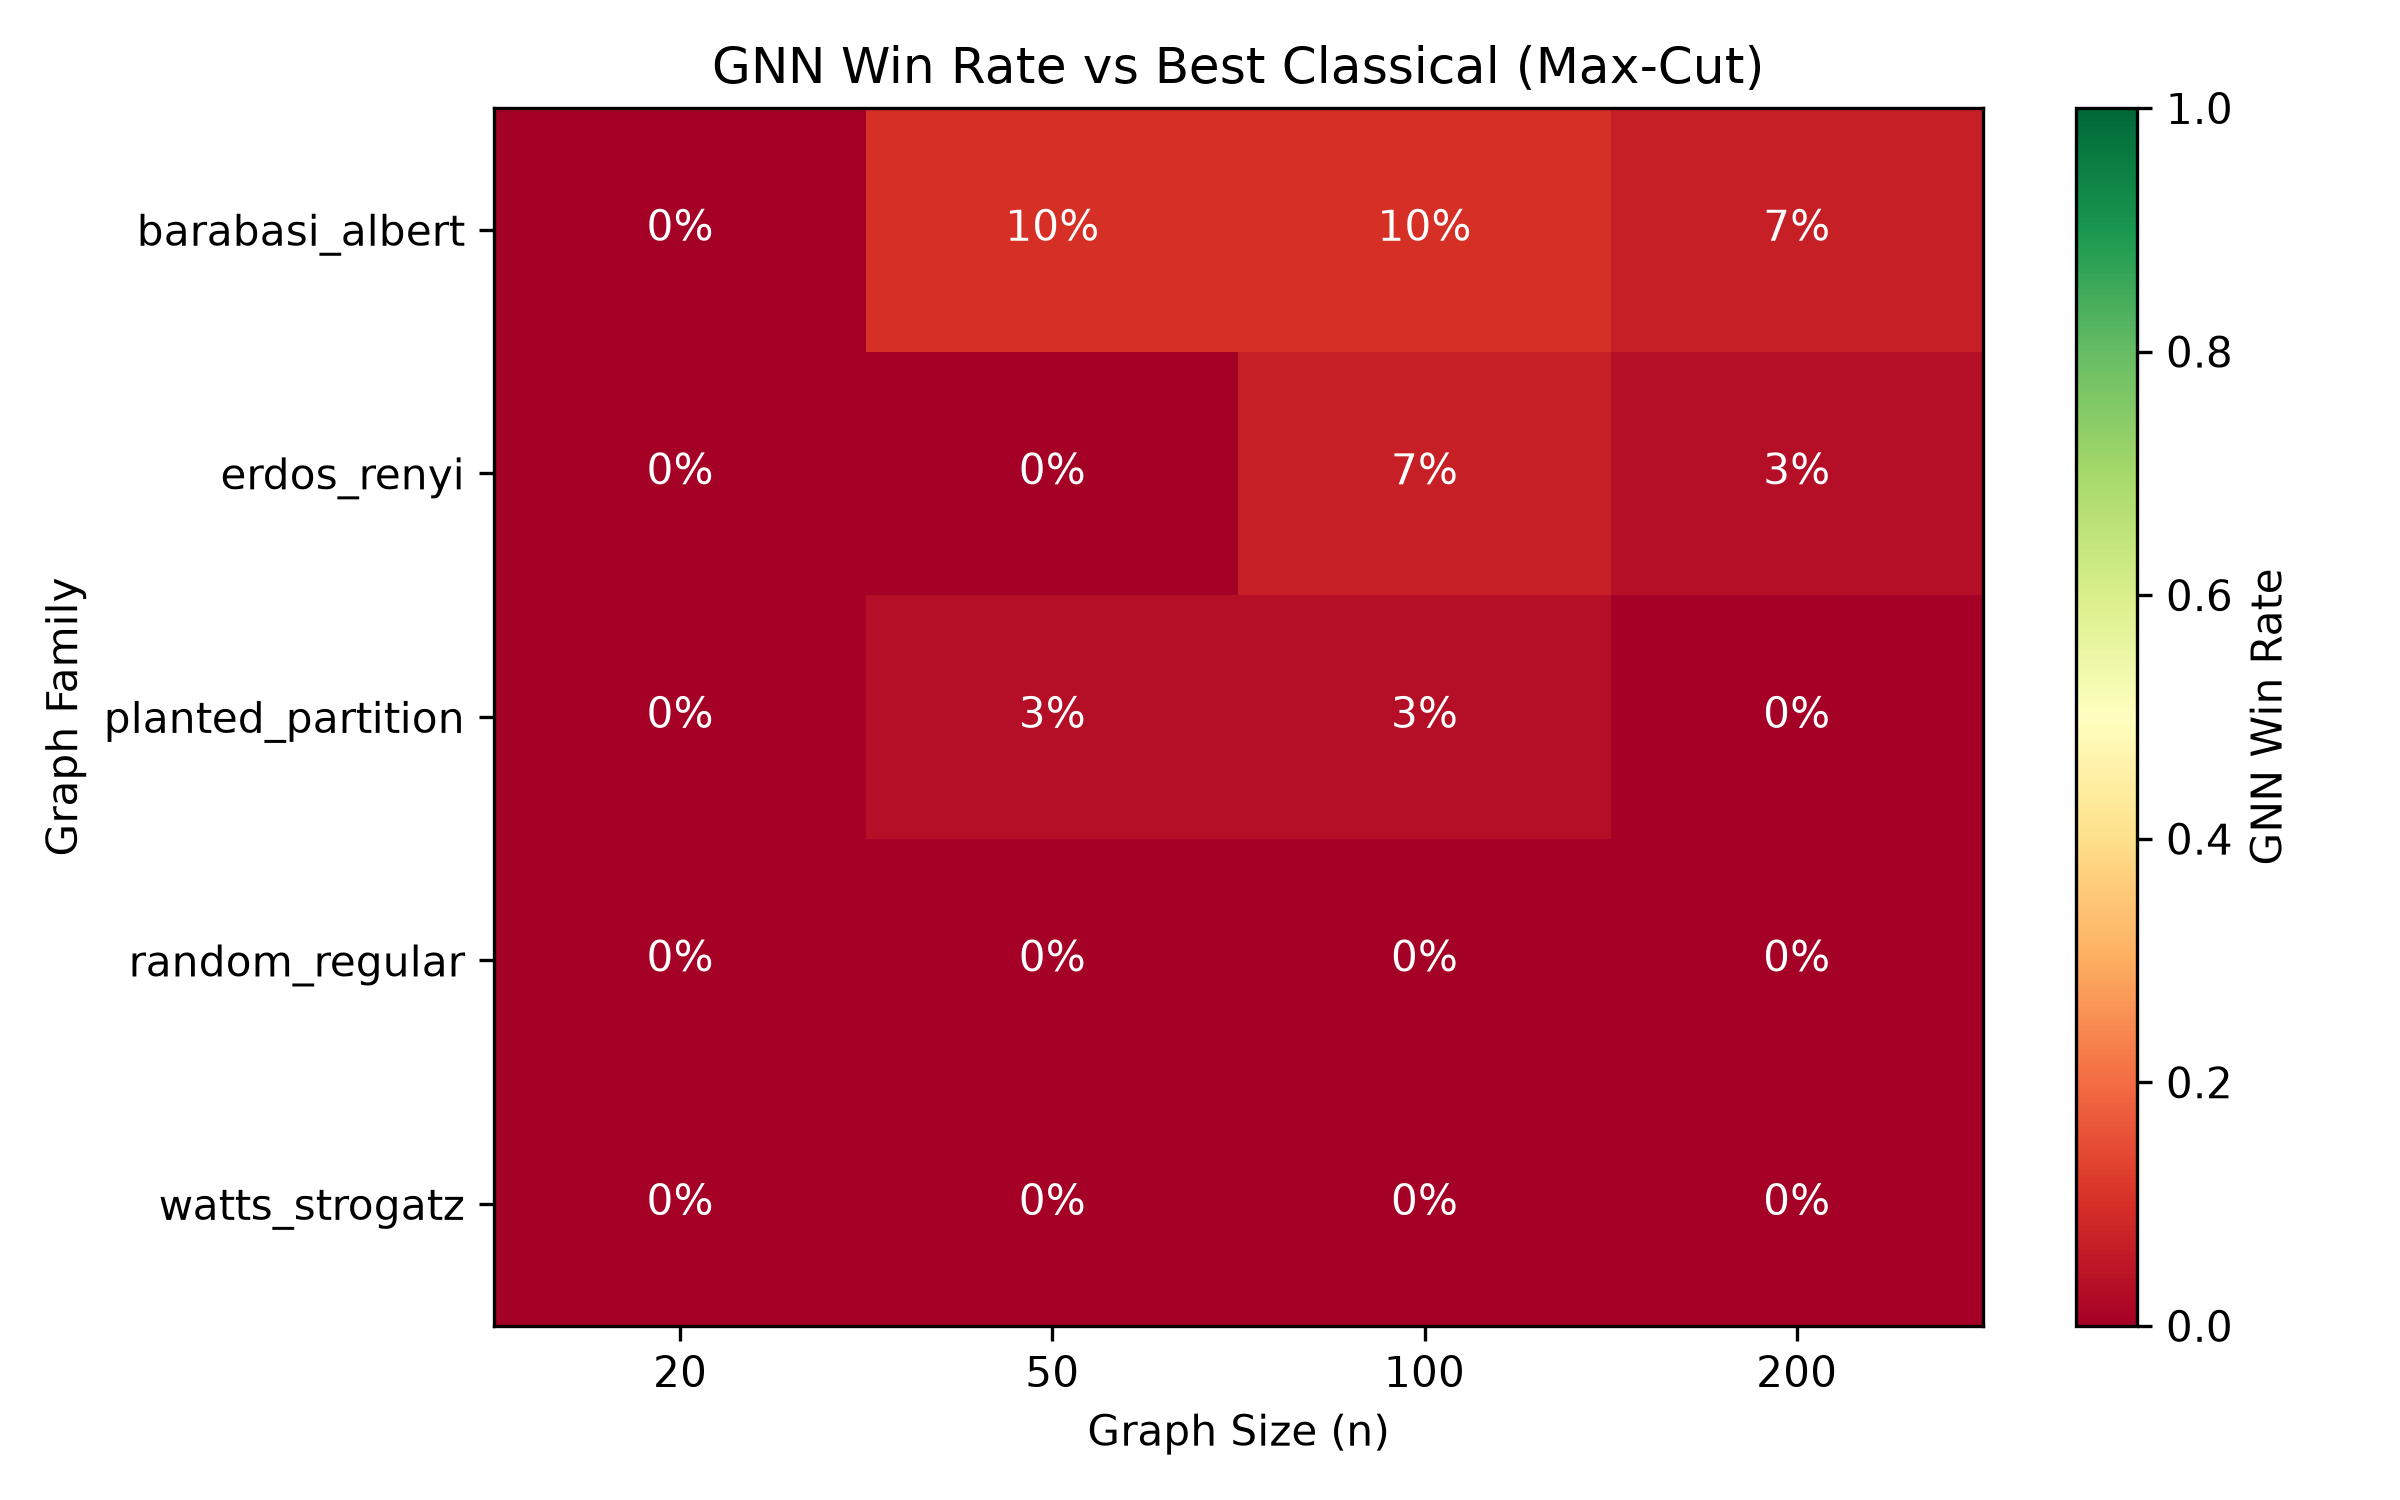
\includegraphics[width=\textwidth]{../analysis/figures/maxcut/win_rate_heatmap.png}
    \caption{GNN win rate by family and size}
\end{subfigure}
\hfill
\begin{subfigure}[b]{0.48\textwidth}
    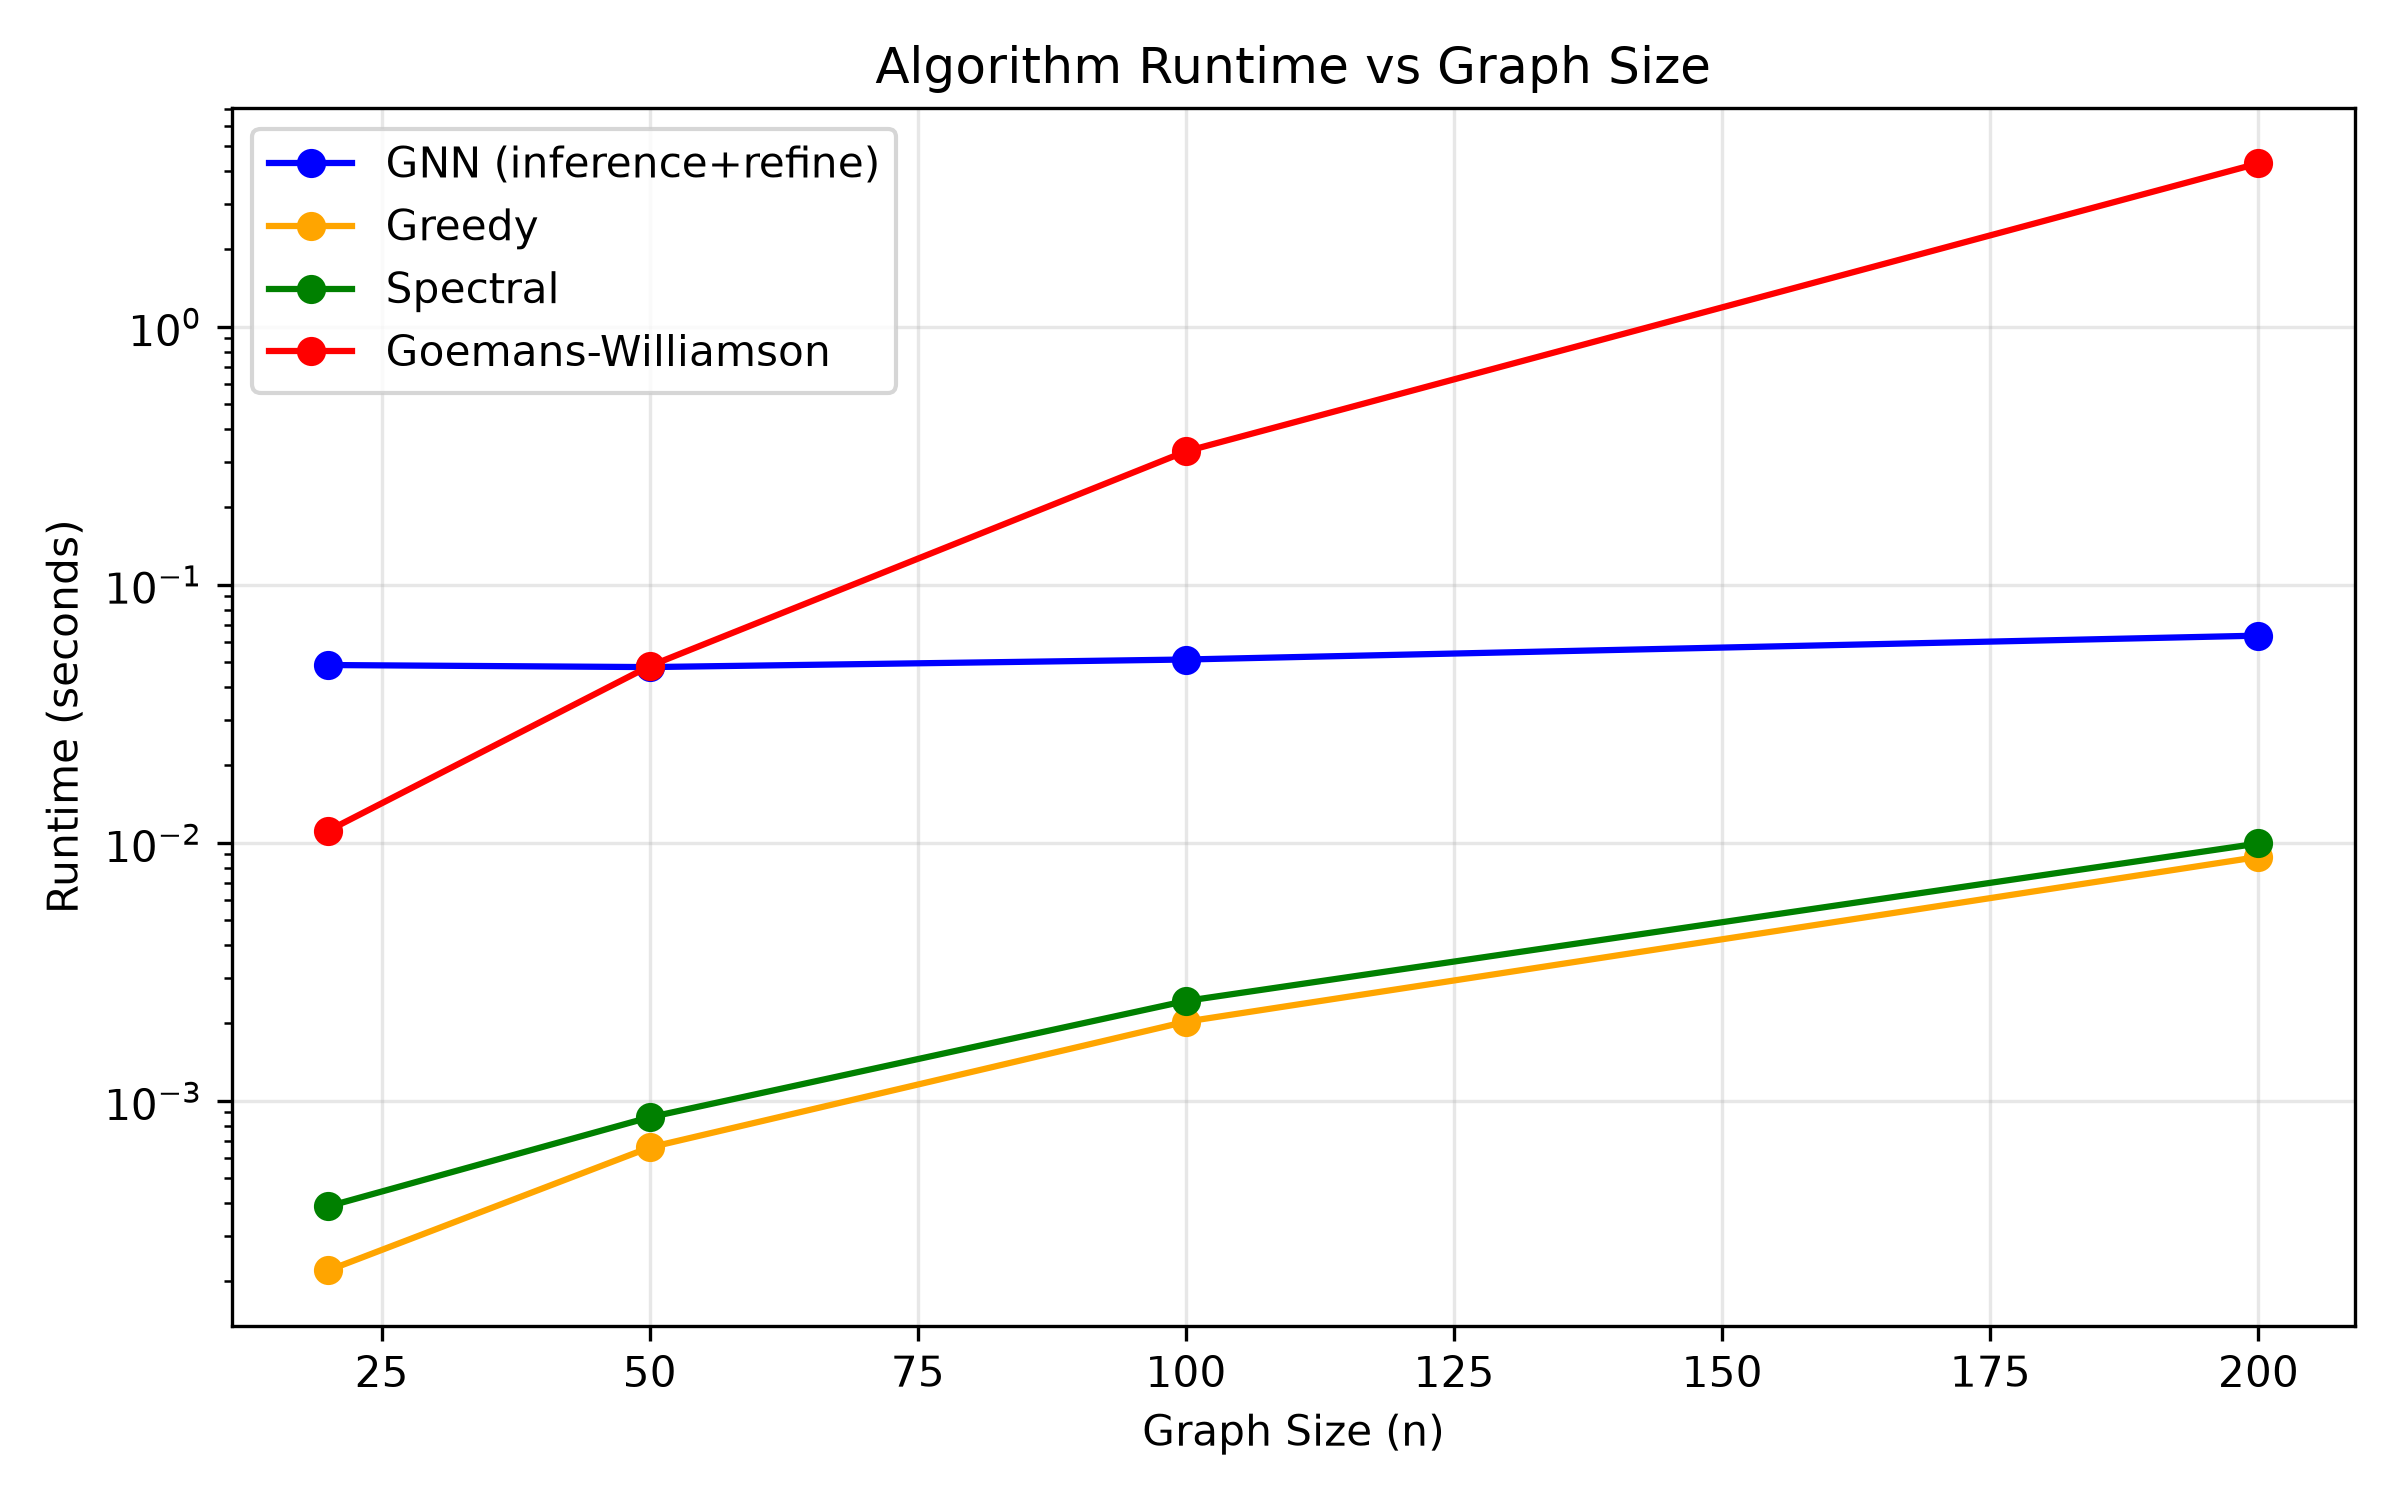
\includegraphics[width=\textwidth]{../analysis/figures/maxcut/runtime_comparison.png}
    \caption{Runtime scaling}
\end{subfigure}
\caption{Max-Cut comparison (rebuilt GNN). The GNN is competitive but does not beat the classical algorithms on quality; its advantage is speed.}
\label{fig:maxcut}
\end{figure}

\subsection{Travelling Salesman Problem}

\begin{table}[h]
\centering
\caption{TSP results on Euclidean instances (3 sizes $\times$ 30 instances = 90 total). Win rate = fraction of instances where the algorithm strictly beats every other algorithm.}
\label{tab:tsp}
\begin{tabular}{lcccc}
\toprule
\textbf{Algorithm} & \textbf{Guarantee} & \textbf{Avg Length/Best} & \textbf{Win Rate} & \textbf{Avg Time (s)} \\
\midrule
Nearest Neighbor & $O(\log n)$ & 1.153 & 0.0\% & $< 0.001$ \\
Christofides & $\leq 1.5$ & 1.056 & 14.4\% & 0.026 \\
NN + 2-opt & --- & \textbf{1.003} & \textbf{85.6\%} & 0.009 \\
\textbf{GNN + 2-opt} & --- & 1.003 & 0.0\% & 0.016 \\
\bottomrule
\end{tabular}
\end{table}

The TSP GNN is trained with proper REINFORCE: a stochastic policy samples the next city from a softmax over embedding-similarity / distance, the log-probability of the sampled tour is computed, and the policy gradient is $\nabla_\theta \log \pi(\text{tour}) \cdot \text{advantage}$.
Despite this, GNN+2-opt produces \emph{identical} tour lengths to NN+2-opt.
Inspection of the trained embeddings (committed with the results) shows why: REINFORCE pushes the policy toward the greedy-scoring optimum, which makes the learned node embeddings mutually parallel---all pairwise cosine similarities equal 1.0 to machine precision---so the greedy score degenerates to $1/\text{dist}$, i.e.\ the GNN collapses to nearest-neighbour.
GNN+2-opt is therefore literally NN+2-opt: the learned initialization contributes nothing, not even as a different starting point.
This suggests that for TSP at this scale, the value of a learned initialization is entirely subsumed by cheap local search, and that a policy-gradient objective with this greedy scoring scheme has no incentive to learn anything beyond nearest-neighbour behaviour.
Christofides achieves tours within 5.6\% of the best (without any local search refinement), confirming its theoretical guarantee of $\leq 1.5 \cdot \text{OPT}$.

\begin{figure}[h]
\centering
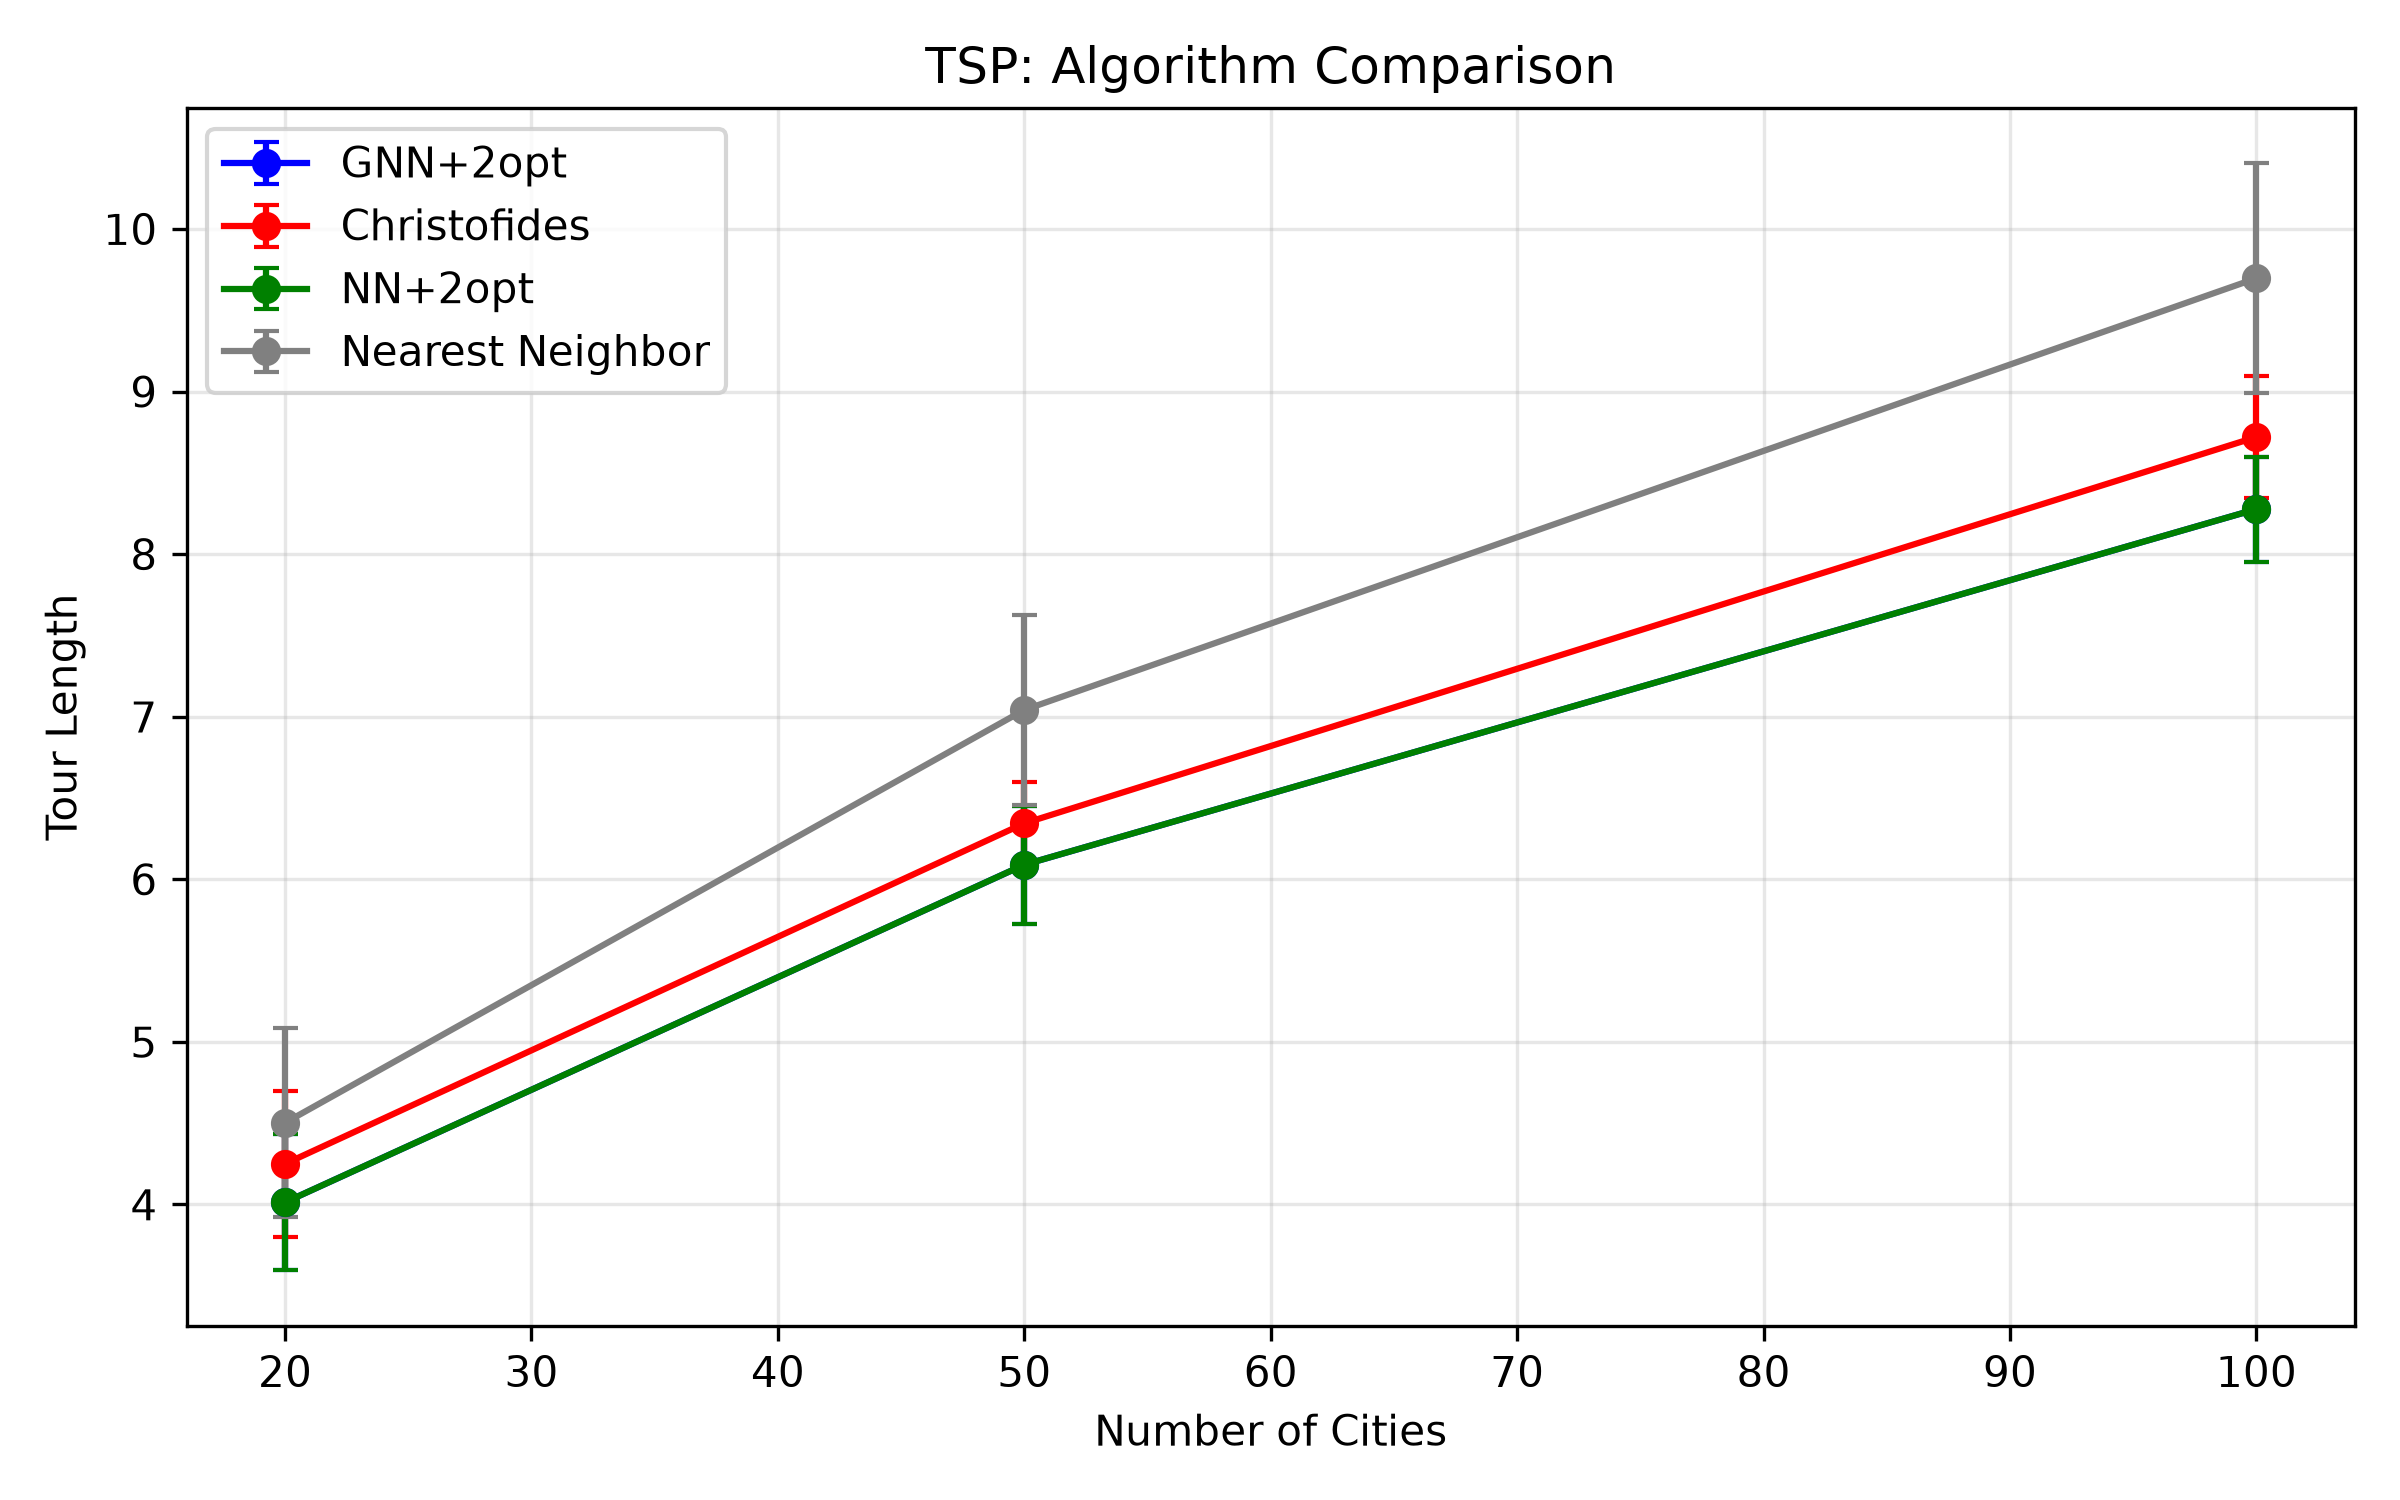
\includegraphics[width=0.7\textwidth]{../analysis/figures/tsp/tsp_comparison.png}
\caption{TSP tour lengths across city counts. GNN+2-opt exactly matches NN+2-opt---the GNN embedding initialization provides no advantage over the simpler nearest neighbor heuristic once 2-opt refinement is applied.}
\label{fig:tsp}
\end{figure}

\subsection{Graph Coloring}

\begin{table}[h]
\centering
\caption{Graph Coloring results across 600 instances. Win rate = fraction of instances where the algorithm strictly beats every other algorithm.}
\label{tab:coloring}
\begin{tabular}{lccc}
\toprule
\textbf{Algorithm} & \textbf{Avg Colors/Best} & \textbf{Win Rate} & \textbf{Avg Time (s)} \\
\midrule
Greedy (random) & 1.280 & 0.0\% & $< 0.001$ \\
Welsh-Powell & 1.136 & 0.0\% & $< 0.001$ \\
DSatur & \textbf{1.000} & \textbf{98.8\%} & 0.005 \\
\textbf{GNN + repair} & 3.388 & 0.0\% & 0.005 \\
\bottomrule
\end{tabular}
\end{table}

Graph coloring is the GNN's worst problem: it uses $3.4\times$ more colors than DSatur on average (mean of per-instance ratios; the ratio of means is $2.8\times$), and wins 0\% of 600 instances across all families and sizes.
This is because coloring is fundamentally a \emph{constraint satisfaction} problem: the objective is to minimize colors while ensuring no adjacent vertices share a color.
The GNN's soft probabilistic output requires post-hoc conflict repair, which greedily introduces additional colors.
DSatur's saturation-based ordering, by contrast, naturally respects the constraint structure.

\begin{figure}[h]
\centering
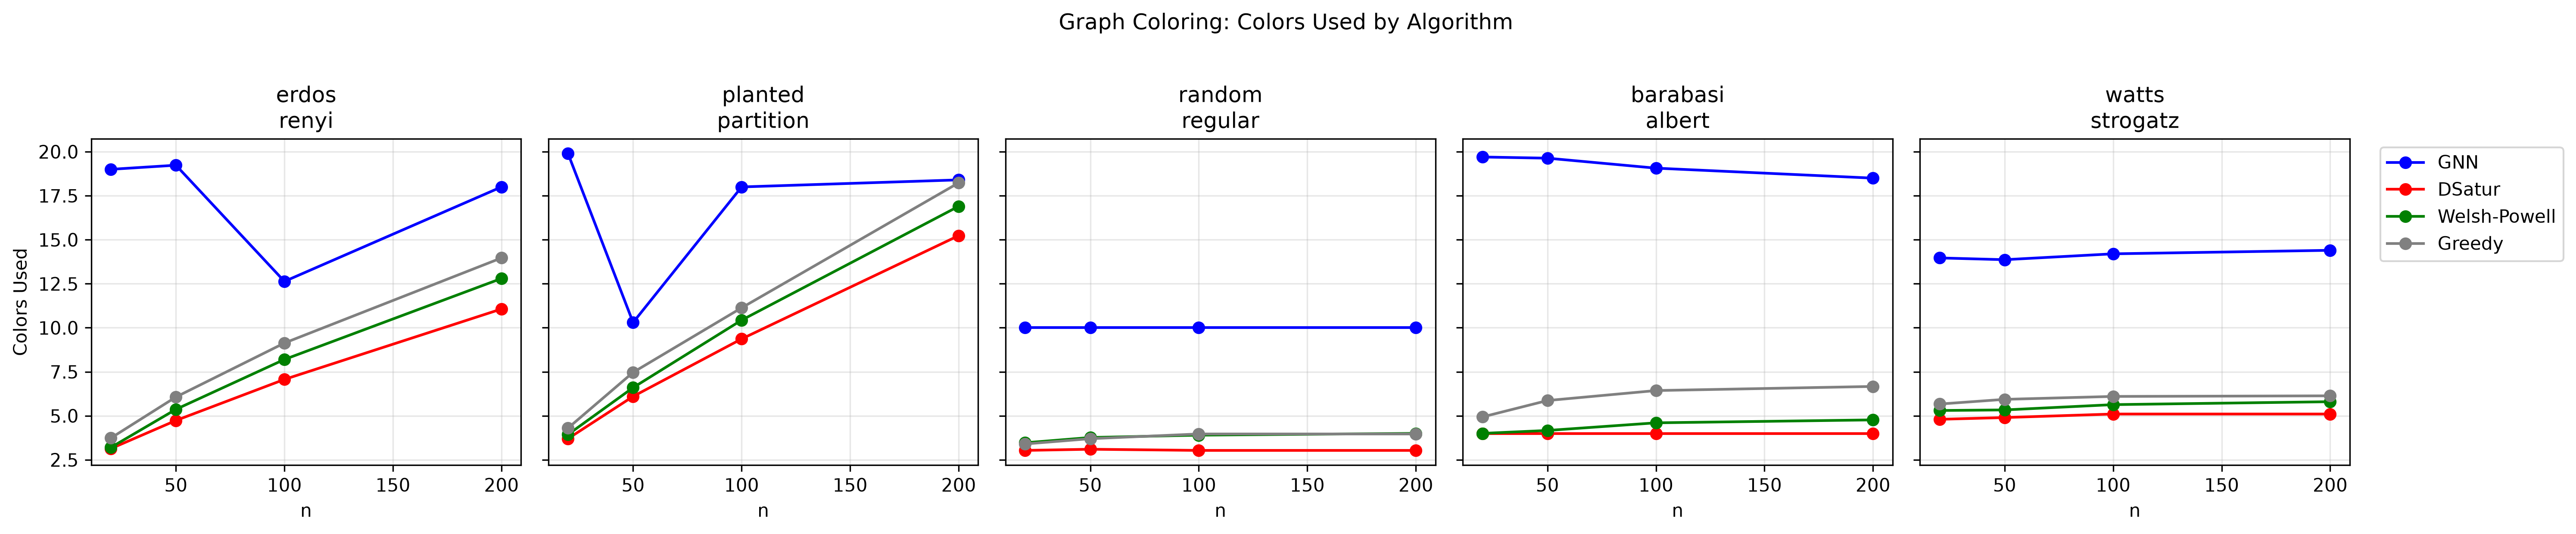
\includegraphics[width=\textwidth]{../analysis/figures/coloring/coloring_comparison.png}
\caption{Colors used by each algorithm across graph families. DSatur consistently uses the fewest colors; the GNN uses $3{-}4\times$ more.}
\label{fig:coloring}
\end{figure}

\subsection{Failure Prediction}

We train logistic regression and random forest classifiers to predict whether the GNN will outperform the best classical algorithm on a given Max-Cut instance, using 12 spectral and structural graph features.

\begin{figure}[h]
\centering
\begin{subfigure}[b]{0.48\textwidth}
    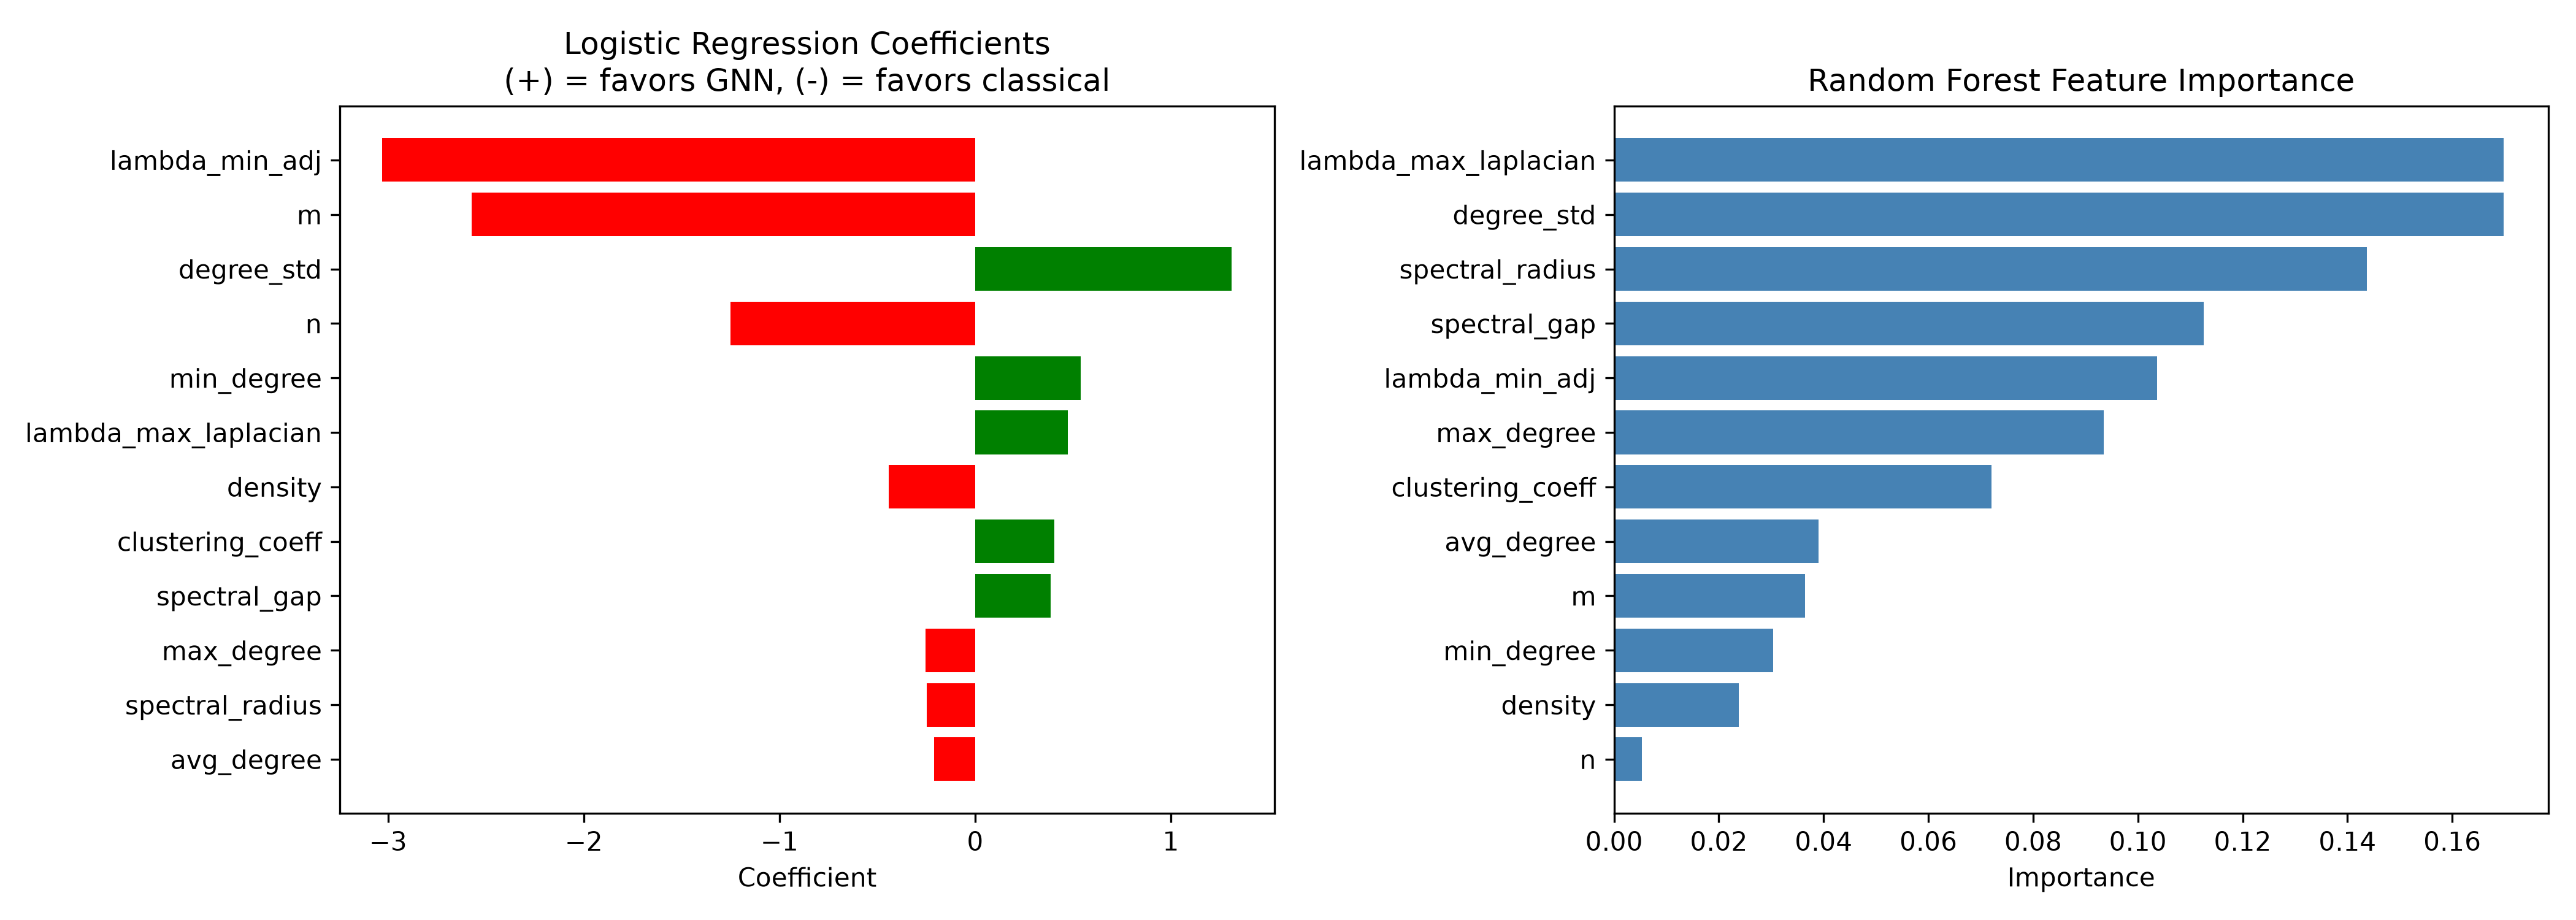
\includegraphics[width=\textwidth]{../analysis/figures/failure_prediction/feature_importance.png}
    \caption{Feature importance for predicting GNN success}
\end{subfigure}
\hfill
\begin{subfigure}[b]{0.48\textwidth}
    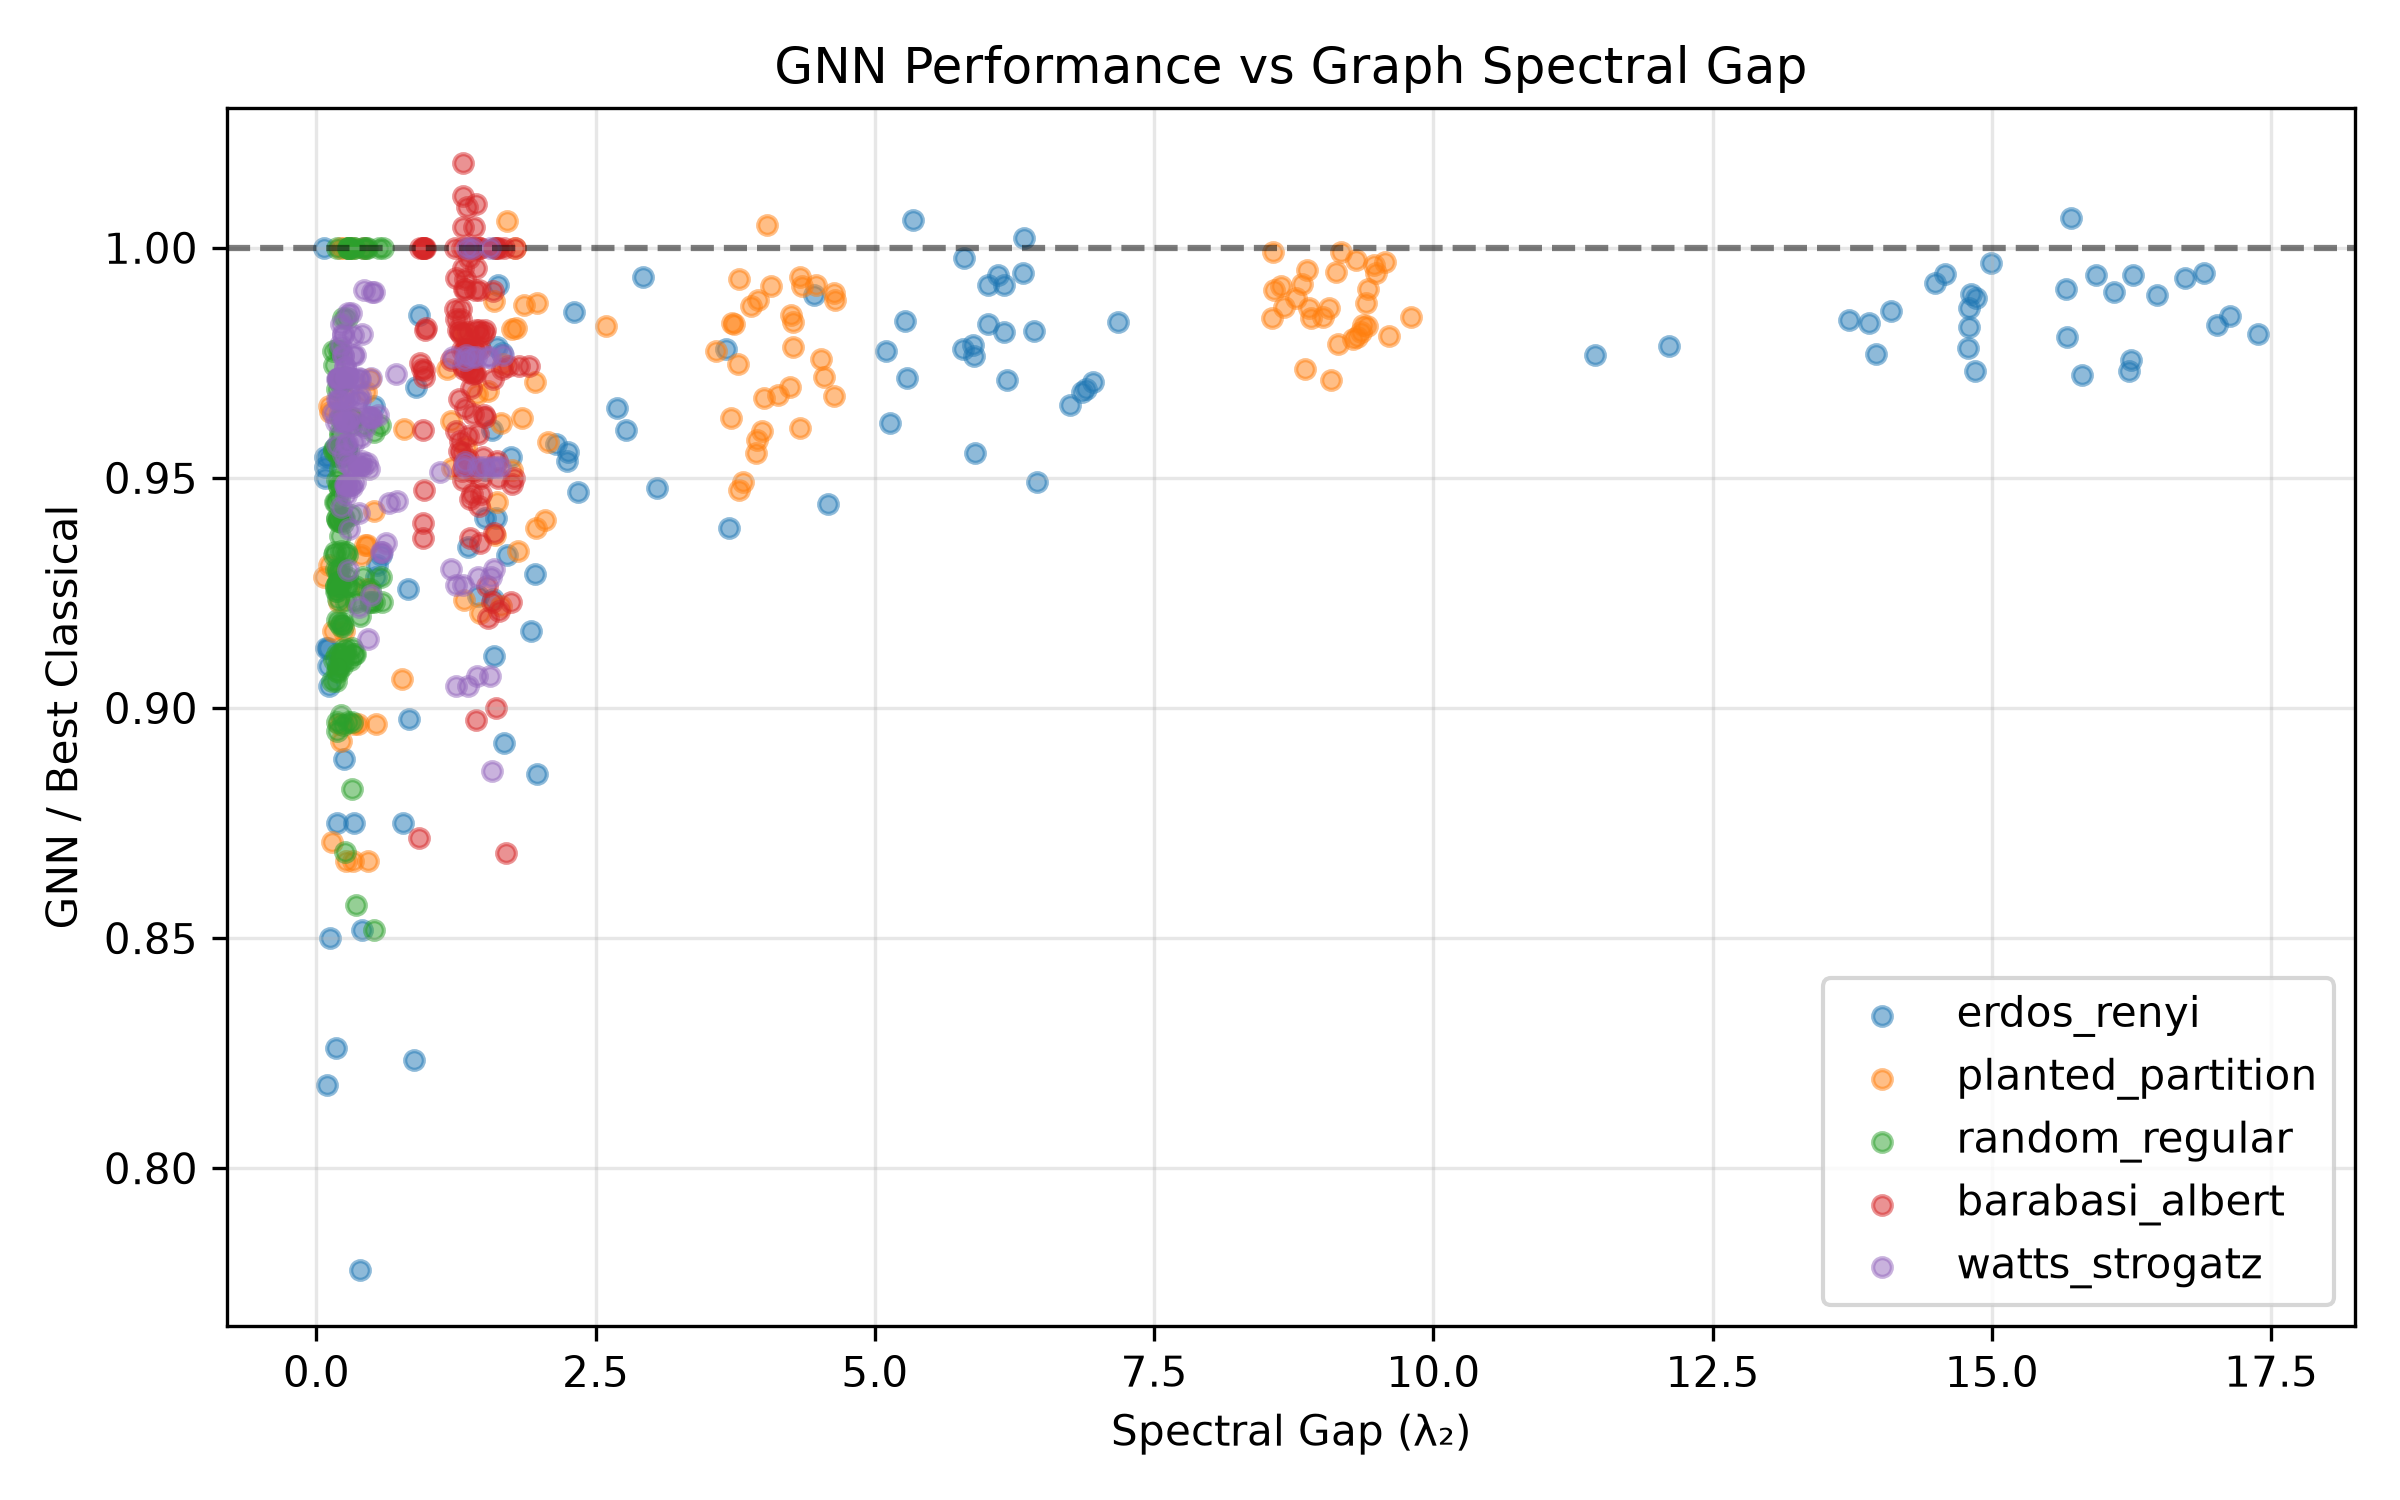
\includegraphics[width=\textwidth]{../analysis/figures/failure_prediction/performance_vs_spectral_gap.png}
    \caption{GNN performance vs.\ spectral gap $\lambda_2$}
\end{subfigure}
\caption{Failure prediction. With 11.3\% positive examples (GNN wins), the majority-class baseline achieves 88.7\% accuracy by always predicting ``classical wins.'' The logistic-regression classifier with balanced class weights achieves balanced accuracy 0.54 and F1 0.21; the random forest 0.47 and 0.16 --- both indistinguishable from chance. The signal is too weak to learn a reliable classifier.}
\label{fig:failure}
\end{figure}

\textbf{Key findings:}
\begin{itemize}
    \item Degree heterogeneity (logistic-regression coefficient $+1.46$ on standardised degree std) and edge count ($-1.42$) are the strongest signed predictors; the random forest leans on the largest Laplacian eigenvalue ($0.158$), the minimum adjacency eigenvalue ($0.114$), degree std ($0.107$), the clustering coefficient ($0.105$) and the spectral gap ($0.100$).
    \item Relative to the best classical cut, the GNN is weakest on planted-partition graphs ($0.981$) and strongest on random-regular graphs ($0.992$) --- the opposite ordering to the original (broken) model, whose degree-blind features could not distinguish regular graphs at all.
    \item \textbf{However}, with 11.3\% positive examples the prediction task is at chance: balanced accuracy 0.54 (LR) / 0.47 (RF), F1 0.21 / 0.16, against a 0.887 majority-class baseline. The learned models are not usable predictors.
\end{itemize}

\section{Discussion}

\subsection{When Should You Use a GNN?}

Our results suggest a clear decision rule:
\begin{enumerate}
    \item \textbf{If solution quality is paramount}: use classical algorithms. The Goemans-Williamson SDP, Christofides, and DSatur all provide stronger solutions with mathematical guarantees.
    \item \textbf{If runtime is the bottleneck}: GNNs offer amortized $O(n)$ inference after training. At $n = 200$, GNN inference was orders of magnitude faster than the GW SDP in the committed run (see Table~\ref{tab:maxcut}); runtimes are environment-dependent.
    \item \textbf{If you need to process millions of instances}: GNNs provide a fast, consistent baseline. But pair them with local search refinement.
\end{enumerate}

\subsection{Why Do GNNs Struggle?}

Four factors explain the GNN's limitations, in rough order of how much they cost on this benchmark:
\begin{enumerate}
    \item \textbf{The objective's geometry.} The unsupervised cut loss is quadratic around the uniform output, with an exact critical point at the random-cut baseline. A model whose features cannot distinguish nodes (constant features) starts on that saddle and barely leaves it; the gradient signal is proportional to the distance from it, so escape is exponentially slow. Symmetry-breaking features plus a non-degenerate initialisation are necessary, not cosmetic.
    \item \textbf{What the refinement contributes.} Local search is not a detail: for the original model it was the entire result, and even for the rebuilt model it supplies most of the quality (raw 0.677 $\to$ refined 0.745). Comparing a refined learned pipeline against unrefined classical baselines measures the refinement, not the learning --- the error this work's ablation exists to correct.
    \item \textbf{Generalisation and expressiveness.} GIN is 1-WL-limited, and the model is trained on one family/size; performance degrades measurably out-of-distribution (0.994 in-distribution vs.\ 0.986 elsewhere). Classical algorithms are instance-agnostic and carry worst-case guarantees.
    \item \textbf{Lack of guarantees.} Even the rebuilt GNN is 1.3\% behind GW on average and has no approximation certificate; GW's SDP objective does, and GW refined is exactly optimal on 299 of the 300 instances verified here.
\end{enumerate}

\subsection{The Role of Local Search}

All GNN solvers in our experiments were refined with local search, and the ablation gives the honest accounting.
For Max-Cut, the original model's refinement was the whole story (coin flip + the same LS = 0.990 of the pipeline); the rebuilt model's raw output is genuinely informative, but the refinement still moves it from 0.677 to 0.745.
For TSP, GNN+2-opt produces \emph{identical} tours to NN+2-opt: the learned initialisation provides zero advantage over nearest-neighbour once local search is applied.
Any comparison of learned and classical solvers must therefore give \emph{both} the same post-processing, or state precisely which side gets it.

\section{Conclusion}

We presented a rigorous empirical comparison of GNN-based solvers against classical approximation algorithms on three NP-hard problems, with an ablation that isolates where performance comes from.
On Max-Cut, a naively-trained GNN was indistinguishable from a coin flip plus the same local search --- and its raw output was worse than a coin flip --- for a provable reason; after the three architectural fixes the network becomes a credible heuristic that beats the coin-flip control and the spectral method but remains 1.3\% behind Goemans-Williamson, whose SDP objective certifies it and which is exactly optimal on 299 of the 300 brute-force-verifiable instances.
On TSP and Graph Coloring the learned solvers lose clearly (TSP collapses to nearest-neighbour; coloring uses 15.4 vs.\ 5.4 mean colours).
Across all three, classical algorithms with proven guarantees remain the reliable baseline, and the learned pipeline's advantage is inference speed, not solution quality.
We also attempted failure prediction from graph features, but with 11.3\% positive examples the task is at chance (LR balanced accuracy 0.54 $\pm$ 0.18, F1 0.21): the GNN wins too rarely to support a reliable classifier, and the majority-class baseline (0.887 raw accuracy) exceeds the learned models in raw accuracy.

These results do not diminish the promise of learned combinatorial solvers---they sharpen its scope.
GNNs are most valuable when speed is critical, when distributional regularity can be exploited, and when paired with classical refinement.
For practitioners, the takeaway is clear: benchmark against the best known algorithms, not just baselines; give every method the same post-processing; and ablate the learned component against a trivial control before attributing performance to it.

\bibliographystyle{plain}
\bibliography{references}

\end{document}
